\documentclass{article}
\usepackage{physics}
\usepackage{graphicx}
\usepackage{caption}
\usepackage{amsmath}
\usepackage{bm}
\usepackage{framed}
\usepackage{authblk}
\usepackage{empheq}
\usepackage{amsfonts}
\usepackage{esint}
\usepackage[makeroom]{cancel}
\usepackage{dsfont}
\usepackage{centernot}
\usepackage{mathtools}
\usepackage{bigints}
\usepackage{amsthm}
\theoremstyle{definition}
\newtheorem{defn}{Definition}[section]
\newtheorem{prop}{Proposition}[section]
\newtheorem{rmk}{Remark}[section]
\newtheorem{thm}{Theorem}[section]
\newtheorem{exmp}{Example}[section]
\newtheorem{prob}{Problem}[section]
\newtheorem{sln}{Solution}[section]
\newtheorem*{prob*}{Problem}
\newtheorem{exer}{Exercise}[section]
\newtheorem*{exer*}{Exercise}
\newtheorem*{sln*}{Solution}
\usepackage{empheq}
\usepackage{tensor}
\usepackage{xcolor}
%\definecolor{colby}{rgb}{0.0, 0.0, 0.5}
\definecolor{MIT}{RGB}{163, 31, 52}
\usepackage[pdftex]{hyperref}
%\hypersetup{colorlinks,urlcolor=colby}
\hypersetup{colorlinks,linkcolor={MIT},citecolor={MIT},urlcolor={MIT}}  
\usepackage[left=1in,right=1in,top=1in,bottom=1in]{geometry}

\usepackage{newpxtext,newpxmath}
\newcommand*\widefbox[1]{\fbox{\hspace{2em}#1\hspace{2em}}}

\newcommand{\p}{\partial}
\newcommand{\R}{\mathbb{R}}
\newcommand{\C}{\mathbb{C}}
\newcommand{\lag}{\mathcal{L}}
\newcommand{\nn}{\nonumber}
\newcommand{\ham}{\mathcal{H}}
\newcommand{\M}{\mathcal{M}}
\newcommand{\I}{\mathcal{I}}
\newcommand{\K}{\mathcal{K}}
\newcommand{\F}{\mathcal{F}}
\newcommand{\w}{\omega}
\newcommand{\lam}{\lambda}
\newcommand{\al}{\alpha}
\newcommand{\be}{\beta}
\newcommand{\x}{\xi}

\newcommand{\G}{\mathcal{G}}

\newcommand{\f}[2]{\frac{#1}{#2}}

\newcommand{\ift}{\infty}

\newcommand{\lp}{\left(}
\newcommand{\rp}{\right)}

\newcommand{\lb}{\left[}
\newcommand{\rb}{\right]}

\newcommand{\lc}{\left\{}
\newcommand{\rc}{\right\}}


\newcommand{\V}{\mathbf{V}}
\newcommand{\U}{\mathcal{U}}
\newcommand{\Id}{\mathcal{I}}
\newcommand{\D}{\mathcal{D}}
\newcommand{\Z}{\mathcal{Z}}

%\setcounter{chapter}{-1}


\usepackage{enumitem}



\usepackage{subfig}
\usepackage{listings}
\captionsetup[lstlisting]{margin=0cm,format=hang,font=small,format=plain,labelfont={bf,up},textfont={it}}
\renewcommand*{\lstlistingname}{Code \textcolor{violet}{\textsl{Mathematica}}}
\definecolor{gris245}{RGB}{245,245,245}
\definecolor{olive}{RGB}{50,140,50}
\definecolor{brun}{RGB}{175,100,80}

%\hypersetup{colorlinks,urlcolor=colby}
\lstset{
	tabsize=4,
	frame=single,
	language=mathematica,
	basicstyle=\scriptsize\ttfamily,
	keywordstyle=\color{black},
	backgroundcolor=\color{gris245},
	commentstyle=\color{gray},
	showstringspaces=false,
	emph={
		r1,
		r2,
		epsilon,epsilon_,
		Newton,Newton_
	},emphstyle={\color{olive}},
	emph={[2]
		L,
		CouleurCourbe,
		PotentielEffectif,
		IdCourbe,
		Courbe
	},emphstyle={[2]\color{blue}},
	emph={[3]r,r_,n,n_},emphstyle={[3]\color{magenta}}
}






\begin{document}
	
\begin{framed}
	\noindent Name: \textbf{Huan Q. Bui}\\
	Course: \textbf{8.309 - Classical Mechanics III}\\
	Problem set: \textbf{\#10}
\end{framed}



\noindent \textbf{1. Classifying Fixed Points.} 
We have the following system
\begin{align*}
&\dot x = x(4+y-x^2)\\
&\dot y = y(x-1)
\end{align*} 
The fixed points satisfy the equations
\begin{align*}
&0 = x(4+y-x^2)\\
&0 = y(x-1)
\end{align*}
We can solve this system by hand, but we can also do this in Mathematica:
\begin{lstlisting}
In[19]:= Solve[{0 == x (4 + y - x^2), 0 == y*(x - 1)}, {x, y}]

Out[19]= {{x -> -2, y -> 0}, {x -> 1, y -> -3}, {x -> 2, 
y -> 0}, {x -> 0, y -> 0}}
\end{lstlisting}
We have four fixed points:
\begin{align*}
(x^*, y^*) \in \{ (\pm 2,0),(1,-3),(0,0) \}
\end{align*}
To study the stability of these fixed points, we need to linearize the system for each point. For each case, we will also diagonalize the dynamical matrix and find its eigenvectors. 

\begin{itemize}
	\item If $(x^*, y^*) = (2,0)$. Linearizing the equations gives
	\begin{align*}
	\dot{\vec{\eta}} = \begin{pmatrix}
	-8 & 2 \\ 0 & 1
	\end{pmatrix} \vec{\eta} \implies \lambda_1 = -8, \lambda_2 = 1 \implies \text{saddle point}
	\end{align*}
	Mathematica code:
	\begin{lstlisting}
	In[28]:= (*Linearize around (2,0)*)
	
	In[29]:= x*(4 + y - x^2) /. {x -> 2 + ex, y -> 0 + ey} // Expand
	
	Out[29]= -8 ex - 6 ex^2 - ex^3 + 2 ey + ex ey
	
	In[30]:= y*(x - 1) /. {x -> 2 + ex, y -> 0 + ey} // Expand
	
	Out[30]= ey + ex ey
	
	In[37]:= Eigensystem[{{-8, 2}, {0, 1}}]
	
	Out[37]= {{-8, 1}, {{1, 0}, {2, 9}}}
	\end{lstlisting}
	
	
	
	
	
	
	\item If $(x^*, y^*) = (-2,0)$. Linearizing the equations gives
	\begin{align*}
	\dot{\vec{\eta}} = \begin{pmatrix}
	-8 & -2 \\ 0 & -3
	\end{pmatrix} \vec{\eta} \implies \lambda_1 = -8, \lambda_2 = -3 \implies \text{stable fixed point}
	\end{align*}
	Mathematica code:
	\begin{lstlisting}
	(*Linearize around (-2,0)*)
	
	In[32]:= x*(4 + y - x^2) /. {x -> -2 + ex, y -> 0 + ey} // Expand
	
	Out[32]= -8 ex + 6 ex^2 - ex^3 - 2 ey + ex ey
	
	In[31]:= y*(x - 1) /. {x -> -2 + ex, y -> 0 + ey} // Expand
	
	Out[31]= -3 ey + ex ey
	
	In[38]:= Eigensystem[{{-8, -2}, {0, -3}}]
	
	Out[38]= {{-8, -3}, {{1, 0}, {-2, 5}}}
	\end{lstlisting}
	
	
	
	\item If $(x^*, y^*) = (0,0)$. Linearizing the equations gives
	\begin{align*}
	\dot{\vec{\eta}} = \begin{pmatrix}
	4 & 0 \\ 0 & -1
	\end{pmatrix} \vec{\eta} \implies  \lambda_1 = -8, \lambda_2 = 1 \implies \text{saddle point}
	\end{align*}
	Mathematica code:
	\begin{lstlisting}
	(*Linearize around (0,0)*)
	
	In[33]:= x*(4 + y - x^2) /. {x -> 0 + ex, y -> 0 + ey} // Expand
	
	Out[33]= 4 ex - ex^3 + ex ey
	
	In[34]:= y*(x - 1) /. {x -> 0 + ex, y -> 0 + ey} // Expand
	
	Out[34]= -ey + ex ey
	
	In[39]:= Eigensystem[{{4, 0}, {0, -1}}]
	
	Out[39]= {{4, -1}, {{1, 0}, {0, 1}}}
	\end{lstlisting}
	
	
	\item If $(x^*, y^*) = (1,-3)$. Linearizing the equations gives
	\begin{align*}
	\dot{\vec{\eta}} = \begin{pmatrix}
	-2 & 1 \\ -3 & 0
	\end{pmatrix} \vec{\eta} \implies \lambda_1 = -3, \lambda_2 = -2 \implies \text{stable fixed point}
	\end{align*}
	Mathematica code:
	\begin{lstlisting}
	(*Linearize around (1,-3)*)
	
	In[35]:= x*(4 + y - x^2) /. {x -> 1 + ex, y -> -3 + ey} // Expand
	
	Out[35]= -2 ex - 3 ex^2 - ex^3 + ey + ex ey
	
	In[36]:= y*(x - 1) /. {x -> 1 + ex, y -> -3 + ey} // Expand
	
	Out[36]= -3 ex + ex ey
	
	In[40]:= Eigensystem[{{-2, 1}, {0, -3}}]
	
	Out[40]= {{-3, -2}, {{-1, 1}, {1, 0}}}
	\end{lstlisting}
\end{itemize}


Sketch of trajectories for this system in the $(x,y)$ plane. The fixed points are marked black. 

\begin{figure}[!htb]
	\centering
	\includegraphics[width=0.3\textwidth]{problem1.eps}
	\caption{Trajectories for this system in the $(x,y)$ plane.}
\end{figure}


Mathematica code:
\begin{lstlisting}
Labeled[Show[
VectorPlot[{x (4 + y - x^2), y (x - 1)}, {x, -4, 4}, {y, -4, 4}],
ListPlot[{{0, 0}, {2, 0}, {-2, 0}, {1, -3}}, 
PlotMarkers -> {Automatic, 15}, 
PlotStyle -> {Thick, Black}]], {"y", "x"}, {Left, Bottom}]
\end{lstlisting}

\newpage

\noindent \textbf{2. Chaos in an Undamped Nonlinear Oscillator.}

\begin{enumerate}[label=(\alph*)]
	\item 
	\begin{figure}[!htb]
		\centering
		\includegraphics[width=0.3\textwidth]{Problem2a.eps}
		\caption{Bifurcation plot showing at least $0.1 < a < 2$. }
	\end{figure}
	There is a window of perioditicity in between the chaotic regions where $a \in (1.25,1.28)$ roughly. We can pick $a = 1.27$.
	\begin{figure}[!htb]
		\centering
		\includegraphics[width=0.3\textwidth]{Problem2a1.eps}
		\caption{Window of perioditicity in between the chaotic regions where $a \in (1.25,1.28)$ roughly. }
	\end{figure}


	\item We first consider $0 < a < 0.1$. 
	\begin{figure}[!htb]
		\centering
		\includegraphics[width=0.4\textwidth]{Problem2b.eps}
		\caption{Bifurcation plot for $0 < a < 0.1$. }
	\end{figure}


	We notice that there is perioditicity for all $a\in (0,0.1)$. To check, we can look at $a \in [0,0.01]$ (see Figure \ref{fig:2b1}). This suggests that we look further. Refering to the first figure, we shall look at the region $a\in [0.35,0.4]$ (see Figure \ref{fig:2b2}). We see that the transition occurs around $\boxed{a = 0.3778}$. To check this, we can look at the Poincare sections and phase portraits for $a = 0.3777$ and $a = 3.779$ (see Figure \ref{fig:2b3}). It is clear that we have a transition from multi-periodic to chaotic as $a$ crosses $0.3778$. 
	
	
	 
	\begin{figure}[!htb]
		\centering
		\includegraphics[width=0.4\textwidth]{Problem2b2.eps}
		\caption{Transition from multi-periodic to chaotic. $a_t\approx 0.3778$. }
		\label{fig:2b2}
	\end{figure}


	\begin{figure}[!htb]
		\centering
		\subfloat[Poincar\'{e} section for chaos at $a=0.3777$]{
			\includegraphics[width=0.3\textwidth]{2b31.eps}
		}
		\subfloat[Phase portrait for chaos at $a=0.3777$.]{
			\includegraphics[width=0.3\textwidth]{2b32.eps}
		}
		\hspace{0mm}
		\subfloat[Poincar\'{e} section for chaos at $a=0.3779$.]{
			\includegraphics[width=0.3\textwidth]{2b33.eps}
		}
		\subfloat[Phase portrait for chaos at $a=0.3779$.]{
			\includegraphics[width=0.3\textwidth]{2b34.eps}
		}
		\caption{Transition from multi-periodic to chaotic as $a$ crosses $0.3778$.}
		\label{fig:2b3}
	\end{figure}
	Finally, just to make sure that there's no chaotic behavior in the region immediately $a = 0.3778$, we could plot a bifurcation diagram for $a\in (0.3776, 0.3777)$. Figure \ref{fig:2b4} shows that YES, the system is still multi-periodic. 
	
	\begin{figure}[!htb]
		\centering
		\includegraphics[width=0.4\textwidth]{2b4.eps}
		\caption{The system is still multi-periodic in $a\in [0.3776, 0.3777]$.}
		\label{fig:2b4}
	\end{figure}
\end{enumerate}



\newpage

\noindent \textbf{3. Bead on a Rotating Hoop.}

\begin{enumerate}[label=(\alph*)]
	\item Let us rescale time so that $\tau = \omega_0 t$ and let $1/\gamma = g/a\omega_0^2$. Let $\theta'$ denote the derivative wrt $\tau$. Then from the original equation, applying the chain rule to change the time derivatives from $dt$ to $d\tau$, we have
	\begin{align*}
	ma \omega_0^2 \theta'' = -\be \omega_0 \theta' + ma\omega_0^2\sin\theta \lp \cos\theta - \f{1}{\gamma}\rp \implies \theta'' = -\f{\be}{ma \omega_0}\theta' + \sin\theta \lp \cos\theta - \f{1}{\gamma}\rp
	\end{align*}
	Finally setting $b = \be / ma \omega_0$ we obtain
	\begin{align*}
	\theta'' = -b \theta' + \sin\theta \lp \cos\theta - \f{1}{\gamma}\rp
	\end{align*}  
	Reverting to the dot convention for time derivatives and setting $\dot \theta = \omega$, we get a system:
	\begin{align*}
	\dot \theta = \omega \quad\text{and} \quad \dot \omega = \sin\theta \lp \cos\theta - \f{1}{\gamma}\rp - b \omega.
	\end{align*}
	This system has a symmetry under $\theta \to -\theta$ and $\omega \to -\omega$. This implies that we have a fixed point $(\theta^*, \omega^*) = (0,0)$. 
	
	
	
	\item The fixed point $(\theta^*, \omega^*) = (0,0)$ always exists. When $b=0$, we may solve the system to get additional fixed points:
	\begin{align*}
	\sin\theta^*\lp \cos\theta^* - \f{1}{\gamma} \rp = 0 \implies \boxed{\theta^* = \pm \arcsec(\gamma) + 2\pi n \quad\text{or}\quad n\pi, \quad\quad n\in \mathbb{Z} }
	\end{align*}
	where the $\arcsec$ solution only exists for $\gamma > 1$. When $b\neq 0$, we don't get additional fixed points since $\omega = 0$ necessarily. To ease of analysis, let us take $n\in \{0,1 \}$ for the $\theta^* = n\pi$ solution and take $n=0$ for the $\arcsec$ solution (if it exists). 
	
	
	Let us now expand $\omega = \omega^* + \epsilon_\omega = \epsilon_\omega$ and $\theta = \theta^* + \epsilon_\theta$. Series expand the sine and cosine we get the linear system:
	\begin{align*}
	&\dot \epsilon_\theta = \epsilon_\omega \\
	&\dot \epsilon_\omega = \cancel{\sin\theta^*\lp \cos\theta^* - \f{1}{\gamma} \rp } + \epsilon_\theta \underbrace{\lp \cos 2 \theta^* - \f{\cos\theta^*}{\gamma}\rp}_{A} -b \epsilon_\omega = A \epsilon_\theta - b \epsilon_\omega.
	\end{align*}
	We have the matrix of coefficients:
	\begin{align*}
	\begin{pmatrix}
	0 & 1 \\ 
	A & -b 
	\end{pmatrix}
	= \begin{pmatrix}
	0 & 1 \\ 
	\cos 2 \theta^* - \f{\cos\theta^*}{\gamma} & -b 
	\end{pmatrix}
	\end{align*}
	If $\theta^* =0$, then we have
	\begin{align*}
	A_{0} = 1 - \f{1}{\gamma}
	\end{align*}
	If $\theta^* = n\pi$, then we have
	\begin{align*}
	A_{1} = 1 + \f{1}{\gamma}
	\end{align*}
	If $\theta^* = \pm \arcsec(\gamma)$, then 
	\begin{align*}
	A_\gamma = \cos (2 \arcsec(\gamma)) - \f{1}{\gamma^2}
	\end{align*}
	We can find the eigensystem for each of these three matrices in Mathematica. For the case $(\theta^*, \omega^*) = (0,0)$, we have
	\begin{align*}
	\lambda_{0,\pm} = \f{-b}{2} \pm \f{1}{2}\sqrt{b^2+4 - \f{4}{\gamma}}
	\end{align*}
	For the case $(\theta^*, \omega^*) = (\pi,0)$ we have
	\begin{align*}
	\lambda_{1,\pm} = \f{-b}{2} \pm \f{1}{2}\sqrt{b^2+4 + \f{4}{\gamma}}.
	\end{align*}
	Finally, for the last case,
	\begin{align*}
	\lambda_{\gamma,\pm} = \f{-b}{2} \pm \f{1}{2\gamma}\sqrt{4 + (b^2-4)\gamma^2}.
	\end{align*}
	Our analysis goes as follows.
	\begin{itemize}
		\item If $b = 0$. There are two subcases:
		\begin{itemize}
			\item If $\gamma < 1$, then the $\pm \arcsec$ fixed points do not exist. Since $4 <  4/\gamma$ in this case, the $(0,0)$ fixed point has purely imaginary associated eigenvalues. The solutions are purely oscillatory, and $(0,0)$ is unstable.  The $(\pi,0)$ fixed point has a positive and a negative eigenvalue, so it is unstable. 
			
			\item If $\gamma > 1$, then the $(\pi ,0)$ fixed point remains unstable, but the $(0,0)$ fixed point becomes stable. The $\pm \arcsec$ fixed points now exist. However, since $4-4\gamma^2 < 0$, these fixed points have purely imaginary associated eigenvalues, and so are unstable. 
		\end{itemize}
		
		
		
		
		
		\item If $b\neq 0$, there are two subcases:
		\begin{itemize}
			\item If $\gamma < 1$, then the $\pm \arcsec$ fixed points do not exist. Since $4 <  4/\gamma$ in this case, the $(0,0)$ fixed point has complex eigenvalues with negative real parts, and so it is a stable fixed point.  The $(\pi,0)$ fixed point has a positive and a negative eigenvalue, so it is unstable. 
			
			\item If $\gamma > 1$, then the $(\pi ,0)$ fixed point remains unstable, but the $(0,0)$ fixed point becomes unstable as well since it now also has a positive and a negative eigenvalue. The $\pm \arcsec$ fixed points now exist. However, since $4-4\gamma^2 < 0$, the associated eigenvalues are complex with  a negative real part,  and so they are stable.  
		\end{itemize}
	\end{itemize}
	
	
	Mathematica code for finding eigenvalues:
	\begin{lstlisting}
	In[95]:= A0 = 1 - (-1)^0/\[Gamma];
	
	In[96]:= A1 = 1 - (-1)^1/\[Gamma];
	
	In[113]:= A\[Gamma] = Cos[2*ArcSec[\[Gamma]]] - 1/\[Gamma]^2;
	
	In[114]:= Eigensystem[{{0, 1}, {A0, -b}}] // FullSimplify
	
	Out[114]= {{-(b/2) - Sqrt[-4 + (4 + b^2) \[Gamma]]/(2 Sqrt[\[Gamma]]),
	1/2 (-b + Sqrt[-4 + (4 + b^2) \[Gamma]]/Sqrt[\[Gamma]])}, {{-((
	2 Sqrt[\[Gamma]])/(
	b Sqrt[\[Gamma]] + Sqrt[-4 + (4 + b^2) \[Gamma]])), 1}, {(
	b \[Gamma] + Sqrt[\[Gamma]] Sqrt[-4 + (4 + b^2) \[Gamma]])/(
	2 (-1 + \[Gamma])), 1}}}
	
	In[115]:= Eigensystem[{{0, 1}, {A1, -b}}] // FullSimplify
	
	Out[115]= {{-(b/2) - Sqrt[4 + (4 + b^2) \[Gamma]]/(2 Sqrt[\[Gamma]]), 
	1/2 (-b + Sqrt[4 + (4 + b^2) \[Gamma]]/Sqrt[\[Gamma]])}, {{(
	b \[Gamma] - Sqrt[\[Gamma]] Sqrt[4 + 4 \[Gamma] + b^2 \[Gamma]])/(
	2 + 2 \[Gamma]), 1}, {(
	b \[Gamma] + Sqrt[\[Gamma]] Sqrt[4 + 4 \[Gamma] + b^2 \[Gamma]])/(
	2 + 2 \[Gamma]), 1}}}
	
	In[116]:= Eigensystem[{{0, 1}, {A\[Gamma], -b}}] // FullSimplify
	
	Out[116]= {{-((b \[Gamma] + Sqrt[4 + (-4 + b^2) \[Gamma]^2])/(
	2 \[Gamma])), (-b \[Gamma] + Sqrt[4 + (-4 + b^2) \[Gamma]^2])/(
	2 \[Gamma])}, {{(\[Gamma] (b \[Gamma] - Sqrt[
	4 + (-4 + b^2) \[Gamma]^2]))/(2 - 2 \[Gamma]^2), 
	1}, {(\[Gamma] (b \[Gamma] + Sqrt[4 + (-4 + b^2) \[Gamma]^2]))/(
	2 - 2 \[Gamma]^2), 1}}}
	\end{lstlisting}
	
	
	
	
	
	
	
	
	
	\item Consider $b=0$. Our system is 
	\begin{align*}
	\dot \theta = \omega \quad\text{and} \quad \dot \omega = \sin\theta \lp \cos\theta - \f{1}{\gamma}\rp - b \omega.
	\end{align*}
	We identify 
	\begin{align*}
	f_\theta(\theta,\omega) = \omega \quad\quad f_\omega(\theta,\omega) = \sin\theta \lp \cos\theta - \f{1}{\gamma}\rp - \cancel{ b \omega}.
	\end{align*}
	The divergence of $\vec{f} = (f_\theta,f_\omega)$ is 
	\begin{align*}
	\div \vec{f} = \f{\p f_\theta}{\p \theta} + \f{\p f_\omega}{\p \omega} =  0
	\end{align*}
	And so the system is conservative. The conserved quantity is 
	\begin{align*}
	\ham(\theta,\omega) 
	&= \int^\omega f_\theta (\theta,\omega')\,d\omega' - \int^\theta f_\omega(\theta',\omega)\,d\theta' \\
	&= \int^\omega \omega'\,d\omega' - \int^\theta \sin\theta' \lp \cos\theta' - \f{1}{\gamma}\rp \,d\theta'\\
	&= \boxed{\f{\omega^2}{2} -  \f{\cos\theta}{\gamma} + \f{\cos^2\theta}{2} }
	\end{align*}
	Mathematica code:
	\begin{lstlisting}
	In[118]:= Integrate[Sin[t]*(Cos[t] - 1/g), t]
	
	Out[118]= Cos[t]/g - Cos[t]^2/2
	\end{lstlisting}
	$\ham(\theta,\omega)$ is not the energy since it is dimensionless. \textbf{\textcolor{blue}{Is it proportional to the energy somehow? I'm running out of time so I won't check this.}}
	
	\begin{figure}[!htb]
		\centering
		\subfloat[$\gamma=3$. Four fixed points. ]{
			\includegraphics[width=0.3\textwidth]{31.eps}
		}
		\subfloat[$\gamma=0.5$. Only two fixed points. ]{
			\includegraphics[width=0.3\textwidth]{32.eps}
		}
		\caption{$\omega$ versus $\theta$. Figure (a): Shown from left to right are the fixed points $(-\arcsec(3),0),(0,0),(\arcsec(3),0),(\pi,0)$. Figure (b): Shown from left to right are the fixed points $(0,0),(\pi,0)$.}
	\end{figure}
	Mathematica code:
	\begin{lstlisting}
	Labeled[Show[
	ContourPlot[
	H1 + Cos[t]/3 - Cos[t]^2/2, {t, -2, 2 Pi}, {w, -Pi, Pi}], 
	ListPlot[{{0, 0}, {Pi, 0}, {ArcSec[3], 0}, {-ArcSec[3], 0}}, 
	PlotStyle -> {Thick, Black}]], {"w", "theta"}, {Left, Bottom}]
	
	Labeled[Show[
	ContourPlot[
	H1 + Cos[t]/0.5 - Cos[t]^2/2, {t, -2, 2 Pi}, {w, -Pi, Pi}], 
	ListPlot[{{0, 0}, {Pi, 0}}, PlotStyle -> {Thick, Black}]], {"w", 
	"theta"}, {Left, Bottom}]
	\end{lstlisting}
	
	
	\item Consider $b=1,\gamma =2$. 
	\begin{figure}[!htb]
		\centering
		\includegraphics[width=0.35\textwidth]{33.eps}
		\caption{$\omega$ versus $\theta$. Instead of solving the equations, we can simply plot the slope field. We see two stable fixed points: the first and third from the left. These are consistent with our analysis from earlier.}
	\end{figure}

	Mathematica code:
	\begin{lstlisting}
	Labeled[Show[
	StreamPlot[{w, Sin[t]*(Cos[t] - 1/2) - w}, {t, -2, 2*Pi}, {w, -4, 
	4}, PerformanceGoal -> "Quality"], 
	ListPlot[{{0, 0}, {Pi, 0}, {ArcSec[2], 0}, {-ArcSec[2], 0}}, 
	PlotStyle -> {Thick, Black}, 
	PlotMarkers -> {Automatic, 10}]], {"w", "theta"}, {Left, Bottom}]
	\end{lstlisting}
	
	
\end{enumerate}


\newpage

\noindent \textbf{4. Bifurcation of a Limit Cycle and Fixed Point}

\begin{enumerate}[label=(\alph*)]
	\item Letting $\dot x = \omega$, we obtain the system: 
	\begin{align*}
	&\dot \omega = -x - a \omega(x^2 + \omega^2 - 1)\\
	&\dot x = \omega
	\end{align*}
	Going into polar coordinates, we have
	\begin{align*}
	r\dot r = x\dot x + \omega \dot \omega \implies 
	r\dot r 
	&= r^2\cos\theta\sin\theta + r\sin\theta (-r\cos\theta - a r\sin\theta (r^2-1)) \\
	&= -ar^2(r^2-1)\sin^2\theta.
	\end{align*}
	Assuming $r>0$ and $a\neq 0$, then we notice that $\dot r = 0$ if $r=1$ and $\theta\in \mathbb{R}$. This shows that there exists a circular limit cycle of radius $r=1$. To find the period of the limit cycle, we use the fact that $x^2 + w^2 = r_\text{limit}^2 = 1$ to find 
	\begin{align*}
	\ddot x = - x \implies x(t) \propto  \cos(t) 
	\end{align*}
	The period is $\boxed{T = 2\pi}$. 
	
	
	
	
	\item To characterize fixed points, we must first find them and then linearize the system of equations. By inspection, it is clear that is only one fixed point $(x^*, \omega^*) = (0,0)$. Now, we linearize the system of equations in Mathematica to find
	\begin{align*}
	&0 = -x - a \omega(x^2 + \omega^2 - 1)\\
	&0 = \omega
	\end{align*}
	gives
	\begin{align*}
	\dot{\vec{\eta}} = \begin{pmatrix}
	-1 & a \\ 0 & 1
	\end{pmatrix}\vec{\eta}
	\end{align*}
	where $\vec{\eta} = (\epsilon_x, \epsilon_\omega)^\top$. The eigenvalues are
	\begin{align*}
	\lambda_{\pm} = \f{1}{2}\lp a \pm \sqrt{a^2-4} \rp
	\end{align*}
	When $a=0$, we get purely imaginary $\lambda$'s. The solution is purely oscillator near the fixed point, which means that the fixed point is unstable. When $a>0$, we have to consider two cases. If $a<2$, the eigenvalues have a positive real part plus an imaginary part, overall giving us growth (plus spiral) as a function of time. In this case the fixed point is unstable. When $a>0$ but $a>2$ also, both eigenvalues are positive, and once again the fixed point is also unstable, but the solution growth exponentially (note that we're talking about a neighborhood of the fixed point here, no limit cycle involved). When $a<0$, we may repeat the same analysis to find that the fixed point becomes stable, as $\lambda_\pm$ are guaranteed to have a negative real part (whether there is a spiral depends on how $\abs{a}$ compares to $2$). 
	
	
	Now we consider the limit cycle. When $a=0$, there are infinitely many limit cycles, so we only consider $a\neq 0$. Suppose $a>0$.  We know that the solutions in the neighborhood of the fixed point $(0,0)$ grow exponentially (therefore) towards the limit cycle. Outside of the limit cycle, however, $w$ tends towards the limit cycle. As a result, the limit cycle is stable for $a>0$. When $a<0$, trajectories from the inside the limit cycle tend towards the origin, while trajectories outside the limit cycle tend away from it, so the limit cycle is unstable. 

	\begin{figure}[!htb]
		\centering
		\subfloat[$a<0$. Unstable limit cycle.]{
			\includegraphics[width=0.35\textwidth]{41.eps}
		}
		\subfloat[$a>0$. Stable limit cycle.]{
			\includegraphics[width=0.35\textwidth]{42.eps}
		}
		\caption{$\omega$ versus $x$. Transition in stability of limit cycle.}
	\end{figure}
	
	
	
	
	\item Going to polar coordinates, we have, as seen in Part (a):
	\begin{align*}
	\dot r = -ar (r^2 - 1)\sin^2\theta
	\end{align*}
	Consider $a>0$. Inside the limit cycle, $r^2 -1 < 0$, and so we have $\dot r > 0 \implies $ trajectories grow out towards the limit cycle. Outside the limit cycle, $r^2 - 1 > 0 \implies \dot r < 0$, and solutions decay towards the limit cycle. So, $a>0$ implies a stable limit cycle. By the exact opposite analysis, we see that $a<0$ implies an unstable limit cycle. \\
	
	We have shown that the system has a limit cycle for all $a\neq 0$. We thus claim that there is a bifurcation point at $a = 0$. As $a$ crosses $0$, the fixed point $(0,0)$ (which always exists) changes stability, so we say that the bifurcation is transcritical. 
	
\end{enumerate}



\noindent \textbf{5. (Optional) \textcolor{blue}{This one seems really cool, but I have 2 more psets to finish before Friday... Although to be honest I have played around with the logistic map and its variants before, so I won't feel like I've missed out on something. }}



\end{document}



